% !TeX program = xelatex
% 本檔新增四組照片／資料圖；原先兩張控制架構圖仍沿用「第二章_插圖片段.tex」。
% 依註解位置分別貼入，不要連續貼在同一小節。
% 這些圖片用於系統介紹，圖說不預設完整任務或實機驗證已完成。

% 建議位置：2.1「移動機械臂平台」的介紹段落後。
本研究使用之移動機械臂模型如\cref{fig:mobile_manipulator_model}所示，由全向移動底盤、六軸機械手臂與末端夾爪組成。底盤提供平面移動能力，手臂與夾爪則用於末端定位及物件互動。
\begin{figure}[htbp]
    \centering
    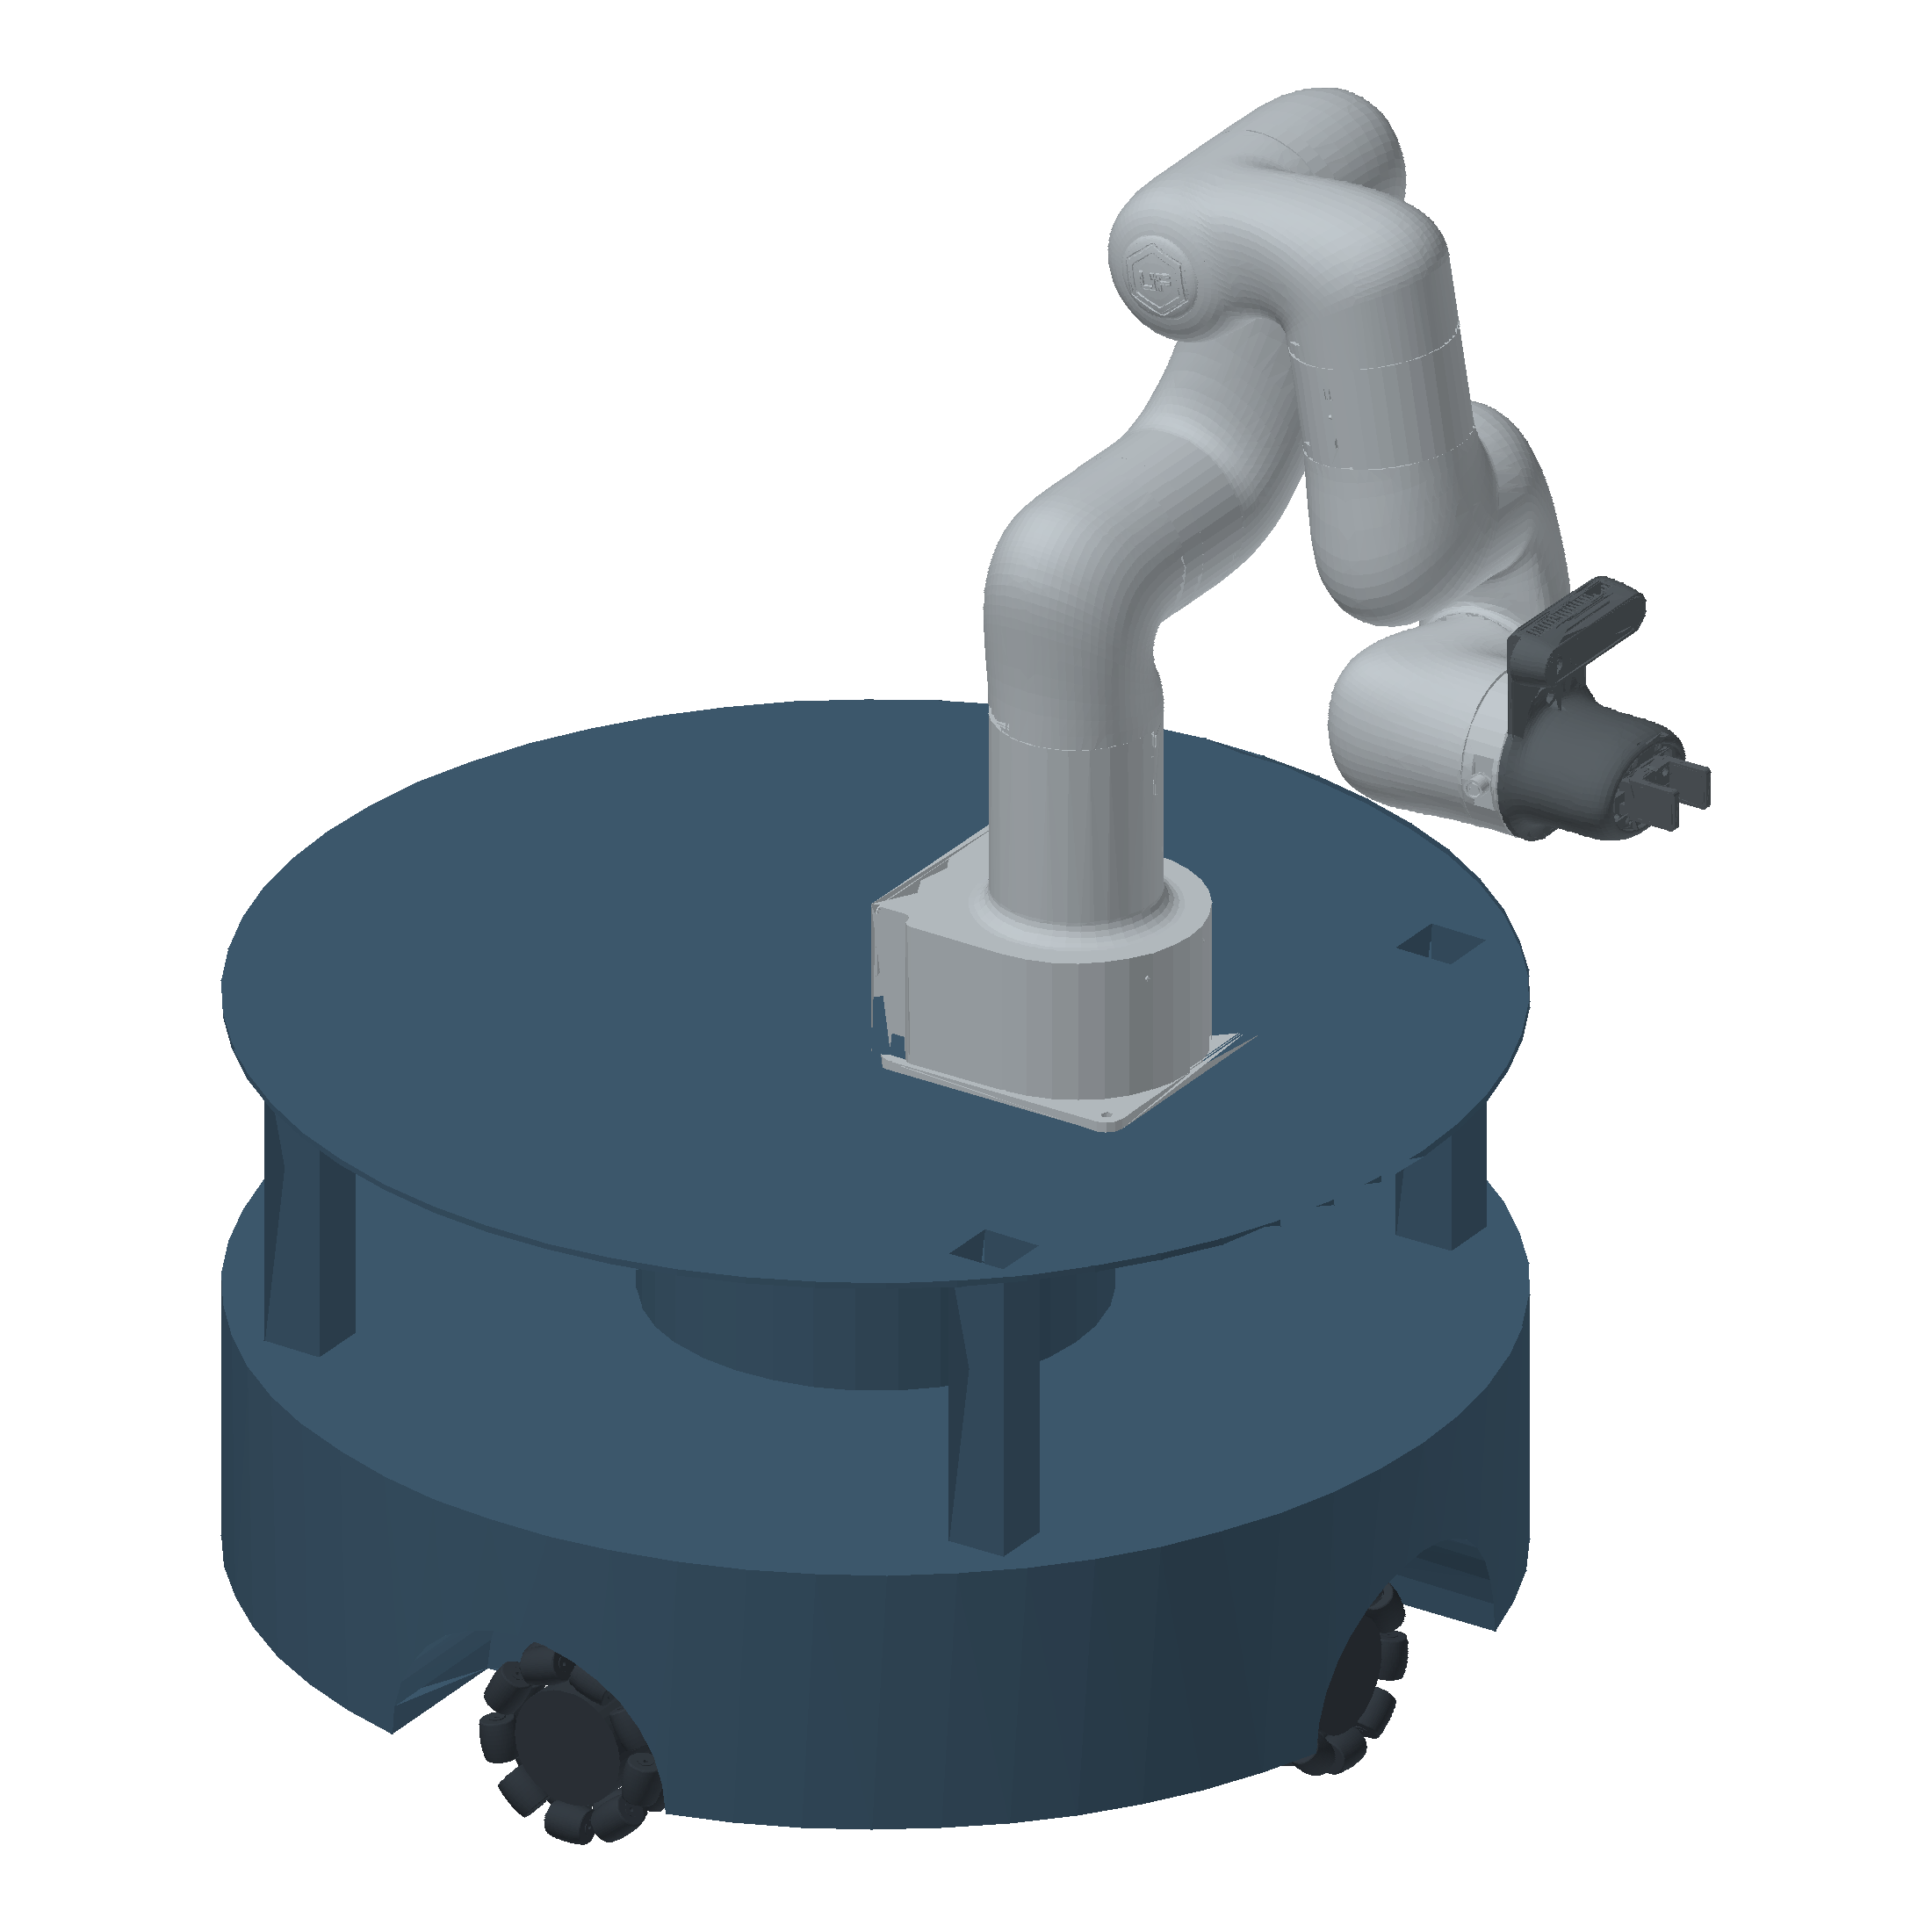
\includegraphics[width=0.53\textwidth]{figsrc/ch02/mobile_manipulator_model.png}
    \caption{移動機械臂之整機模型示意}
    \label{fig:mobile_manipulator_model}
\end{figure}

% 建議位置：2.2.1「雷射掃描與深度相機」，說明手腕相機配置的段落後。
手腕相機與夾爪之相對配置如\cref{fig:wrist_camera_gripper_model}所示。相機隨手臂運動改變觀測位置，影像量測需配合對應時刻的機器人狀態進行座標轉換，才能形成控制端使用的操作目標。
\begin{figure}[htbp]
    \centering
    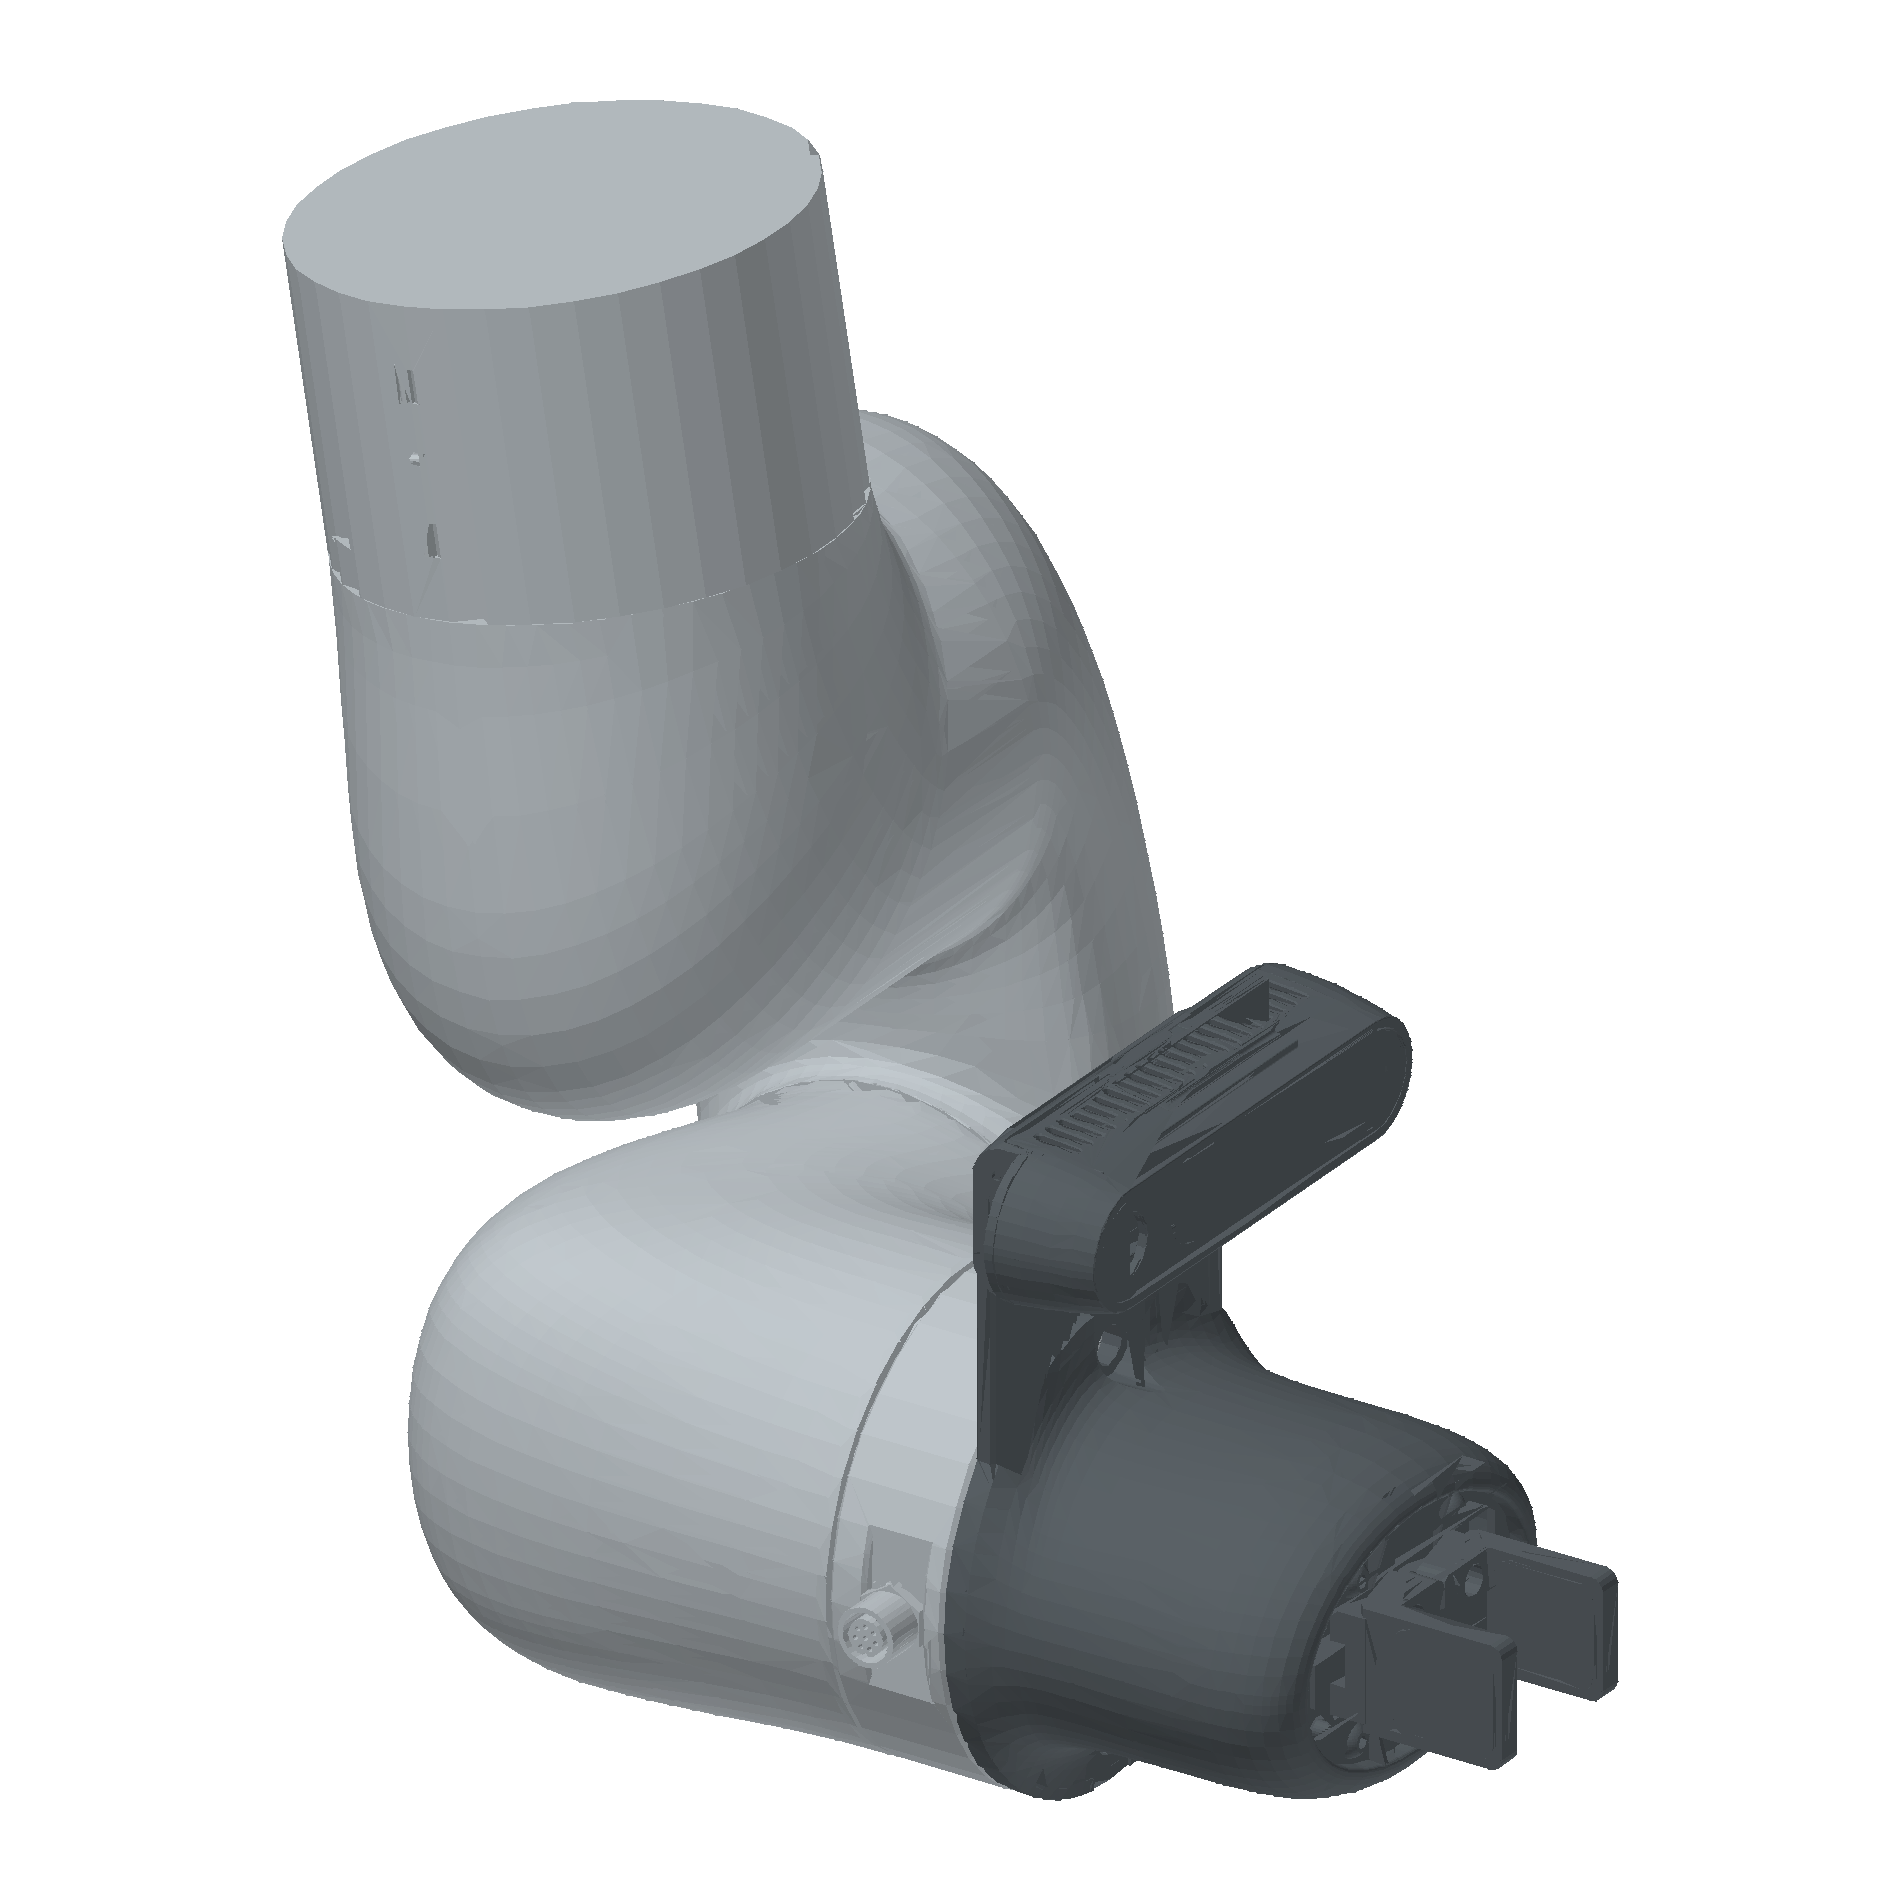
\includegraphics[width=0.47\textwidth]{figsrc/ch02/wrist_camera_gripper_model.png}
    \caption{手腕相機與末端夾爪之模型配置}
    \label{fig:wrist_camera_gripper_model}
\end{figure}

% 建議位置：2.3.2「Isaac Sim 物理模擬與場景建置」，說明場景配置的段落後。
模擬環境依任務配置門扇、牆面、桌面及操作物件，如\cref{fig:isaac_task_areas}所示。門區域用於建立機構操作與通行的研究情境，桌邊區域則用於物件接近與抓取；圖中畫面取自既有模擬紀錄的狀態重播。
\begin{figure}[htbp]
    \centering
    \begin{minipage}[b]{0.49\textwidth}
        \centering
        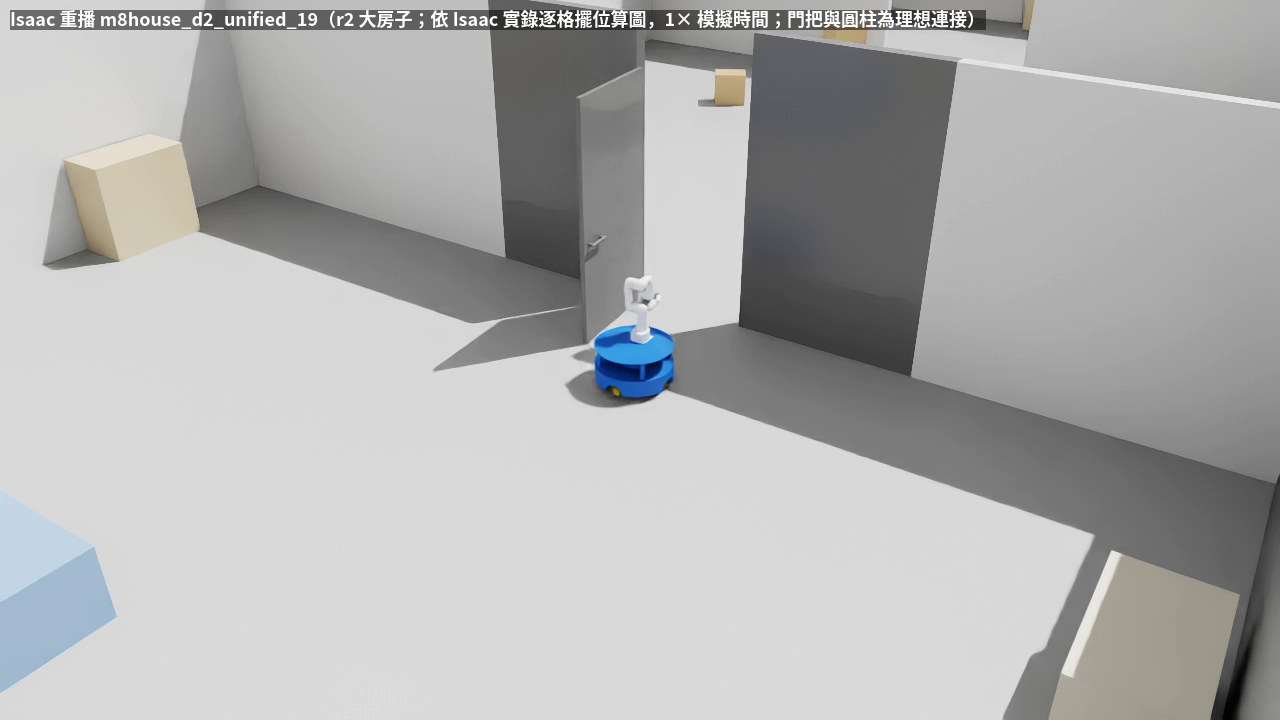
\includegraphics[width=\linewidth]{figsrc/ch02/isaac_door_area.png}
        \par\smallskip
        {\small (a) 門與通行區域}
    \end{minipage}\hfill
    \begin{minipage}[b]{0.49\textwidth}
        \centering
        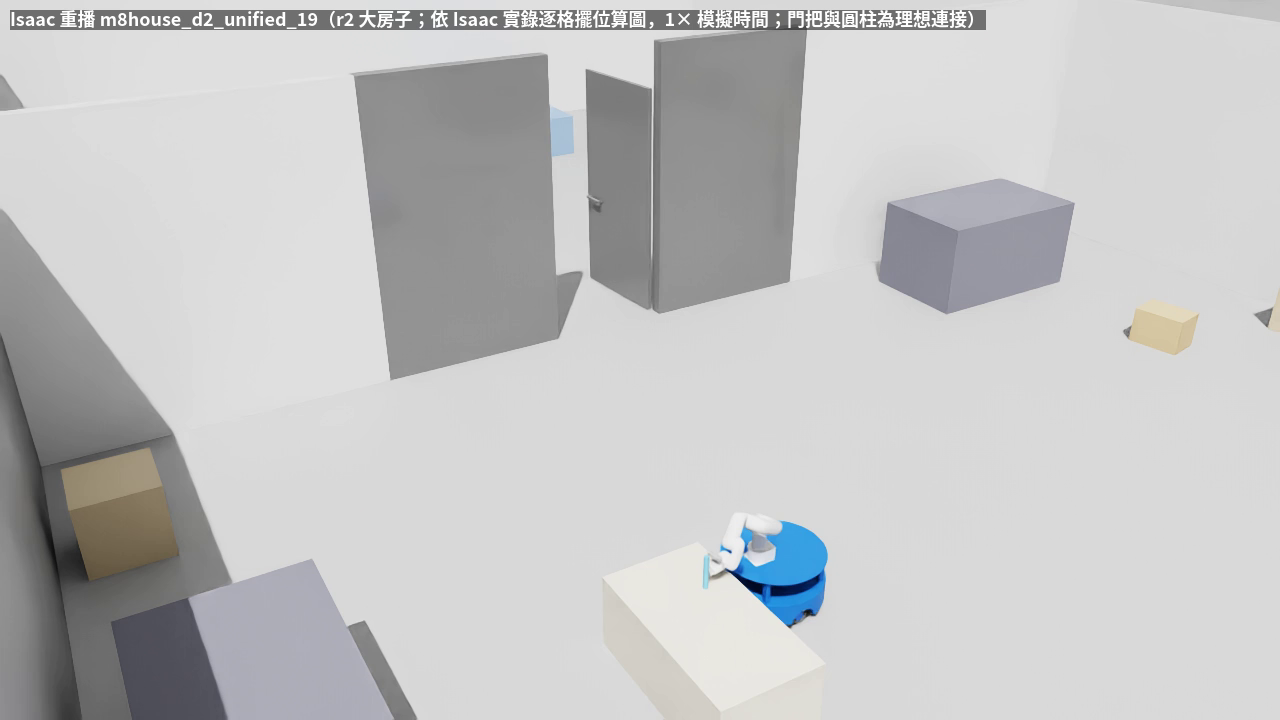
\includegraphics[width=\linewidth]{figsrc/ch02/isaac_table_area.png}
        \par\smallskip
        {\small (b) 桌邊取物區域}
    \end{minipage}
    \caption{Isaac Sim 模擬場景之門與桌邊取物區域}
    \label{fig:isaac_task_areas}
\end{figure}

% 建議位置：2.4.2「視覺感知與操作目標資訊」，說明 RGB-D 量測的段落後。
門把手觀測之 RGB 影像與對應深度資料如\cref{fig:door_handle_rgbd}所示。彩色影像提供物件外觀與影像位置，深度資料則提供相機至場景表面的距離資訊；兩者共同支援後續的三維目標定位。
\begin{figure}[htbp]
    \centering
    \begin{minipage}[b]{0.49\textwidth}
        \centering
        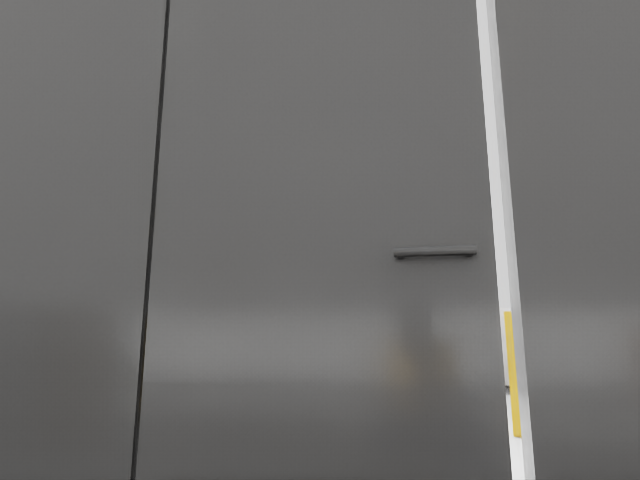
\includegraphics[width=\linewidth,height=4.0cm,keepaspectratio]{figsrc/ch02/door_handle_rgb.png}
        \par\smallskip
        {\small (a) RGB 影像}
    \end{minipage}\hfill
    \begin{minipage}[b]{0.49\textwidth}
        \centering
        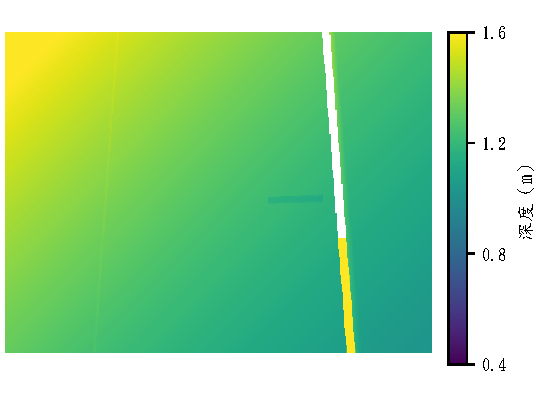
\includegraphics[width=\linewidth,height=4.0cm,keepaspectratio]{figsrc/ch02/door_handle_depth.pdf}
        \par\smallskip
        {\small (b) 對應深度影像}
    \end{minipage}
    \caption{門把手之 RGB 與對應深度觀測示例；深度圖以公尺表示，白色為無效深度}
    \label{fig:door_handle_rgbd}
\end{figure}
